% Created 2023-12-03 So 16:34
% Intended LaTeX compiler: pdflatex
\documentclass[11pt]{article}
\usepackage[utf8]{inputenc}
\usepackage{lmodern}
\usepackage[T1]{fontenc}
\usepackage{textcomp}
\usepackage{graphicx}
\usepackage{longtable}
\usepackage{wrapfig}
\usepackage{rotating}
\usepackage[normalem]{ulem}
\usepackage{amsmath}
\usepackage{amssymb}
\usepackage{capt-of}
\usepackage{hyperref}
\usepackage{verbatim}
\usepackage{listings}
\usepackage{underscore}
\author{Leon Schwarzäugl}
\date{\today}
\title{Computational Science on Many-Core Architectures \\Exercise 7}
\hypersetup{
 pdfauthor={Leon Schwarzäugl},
 pdftitle={Computational Science on Many-Core Architectures, Exercise 7},
 pdfkeywords={},
 pdfsubject={},
 pdfcreator={Emacs 30.0.50 (Org mode 9.6.12)},
 pdflang={English}}
\begin{document}
\maketitle
The code for all tasks can be found at: \url{https://github.com/Swarsel/CSE_TUWIEN/tree/main/WS2023/Many-Core%20Architectures/e7}

\newpage
\section{Pipelined Conjugate Gradients}

I implemented the pipelined conjugate gradients using the two kernels introduced in the lecture:

\begin{small}
\begin{verbatim}

__global__ void XRP(double *solution, double *p, double* r, double* Ap, double* result,
                            int N, double alpha, double beta) {
  double dot{0};
  for (int i = blockIdx.x * blockDim.x + threadIdx.x; i < N; i += blockDim.x * gridDim.x){
    solution[i] += alpha * p[i];
    r[i] -= alpha * Ap[i];
    p[i] = r[i] + beta * p[i];
    dot += r[i] * r[i];
  }
  for (int j=warpSize/2; j>0; j=j/2) {
    dot += __shfl_xor_sync(0xffffffff, dot, j);
  }

  if (threadIdx.x % warpSize == 0) {
    atomicAdd(result, dot);
  }}

__global__ void API(int N, int *csr_rowoffsets, int *csr_colindices, double *csr_values,
                           double *p, double *Ap, double *result_pAp, double *result_ApAp) {
  double pAp{0}, ApAp{0};
  for (int row = blockIdx.x * blockDim.x + threadIdx.x; row < N; row += blockDim.x * gridDim.x) {
    double sum = 0;
    for (int jj = csr_rowoffsets[row]; jj < csr_rowoffsets[row + 1]; ++jj) {
      sum += csr_values[jj] * p[csr_colindices[jj]];
    }
    Ap[row] = sum;
    pAp += p[row] * Ap[row];
    ApAp += Ap[row] * Ap[row];
  }

  for (int j=warpSize/2; j>0; j=j/2) {
    pAp += __shfl_xor_sync(0xffffffff, pAp, j);
    ApAp += __shfl_xor_sync(0xffffffff, ApAp, j);
  }

  if (threadIdx.x % warpSize == 0) {
    atomicAdd(result_pAp, pAp);
    atomicAdd(result_ApAp, ApAp);
  }}
\end{verbatim}
\end{small}

The CG algorithm itself was adjusted to perform one initial calculation of \(\alpha_0, \beta_0, Ap_0\) using the `old' kernels and then use the more efficient kernels for the rest of the iterations:

\begin{small}
\begin{verbatim}

[...]

  cuda_csr_matvec_product<<<512, 512>>>(N, csr_rowoffsets, csr_colindices, csr_values, cuda_p, cuda_Ap);

  cudaMemcpy(cuda_scalar, &zero, sizeof(double), cudaMemcpyHostToDevice);
  cudaMemcpy(cuda_scalar2, &zero, sizeof(double), cudaMemcpyHostToDevice);
  cuda_dot_product<<<512, 512>>>(N, cuda_p, cuda_Ap, cuda_scalar);
  cuda_dot_product<<<512, 512>>>(N, cuda_Ap, cuda_Ap, cuda_scalar2);
  cudaMemcpy(&alpha, cuda_scalar, sizeof(double), cudaMemcpyDeviceToHost);
  cudaMemcpy(&beta, cuda_scalar2, sizeof(double), cudaMemcpyDeviceToHost);
  alpha = residual_norm_squared / alpha;
  beta = alpha*alpha*beta / residual_norm_squared - 1;

  int iters = 0;
  cudaDeviceSynchronize();
  timer.reset();
  while (1) {

    cudaMemcpy(cuda_scalar, &zero, sizeof(double), cudaMemcpyHostToDevice);
    cudaMemcpy(cuda_scalar2, &zero, sizeof(double), cudaMemcpyHostToDevice);
    XRP<<<512, 512>>>(cuda_solution, cuda_p, cuda_r, cuda_Ap, cuda_scalar, N, alpha, beta);
    cudaMemcpy(&residual_norm_squared, cuda_scalar, sizeof(double), cudaMemcpyDeviceToHost);
    cudaMemcpy(cuda_scalar, &zero, sizeof(double), cudaMemcpyHostToDevice);
    API<<<512, 512>>>(N, csr_rowoffsets, csr_colindices, csr_values, cuda_p, cuda_Ap, cuda_scalar, cuda_scalar2);
    cudaMemcpy(&alpha, cuda_scalar, sizeof(double), cudaMemcpyDeviceToHost);
    cudaMemcpy(&beta, cuda_scalar2, sizeof(double), cudaMemcpyDeviceToHost);
    alpha = residual_norm_squared / alpha;
    beta = (alpha*alpha*beta / residual_norm_squared) - 1;

[...]

\end{verbatim}
\end{small}
\pagebreak

Using what we learned this and last week, I had four different versions of (Assembly, CG) at my disposal for benchmarking. Below are the results.
\\
As always, each system size was ran 14 times, with the lowest and highest 2 times omitted before averaging over the rest.

First, the results with all four systems compared against each other:

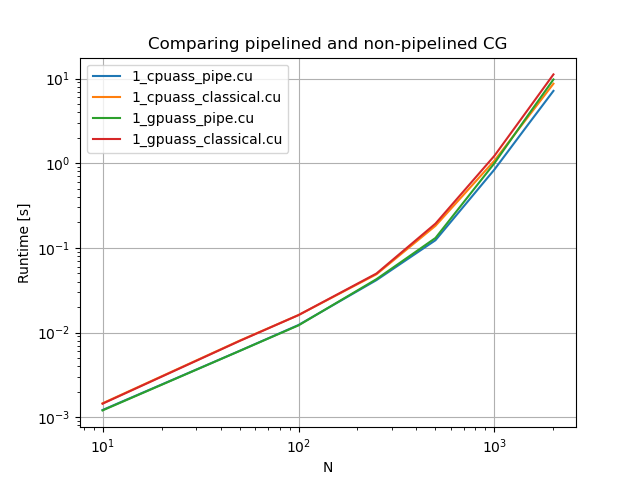
\includegraphics[scale=0.8]{plots/1comp_quad.png}

(The x-axis is wrongly labeled as \(N\) here, it should read \(\sqrt{N}\).) \\
I have to say that I am disappointed with the GPU matrix assembly results - after last weeks results, I thought I would reach way better runtimes here. But it seems not to be the case here. Interestingly, the GPU assembled implementation really takes off in runtime (in a bad way) for high \(N\), even taking longer than the classical implementation then. Maybe I introduced a bug while transporting the pipelined implementation into the GPU assembly framework, but at least I could not find it.

Anyways, what we actually wanted to show here holds - that is, the pipelined implementations are a lot faster than the classical implementations. To get a better picture of this distinction, I ran another benchmark with more system sizes only comparing the CPU assembly versions against each other:

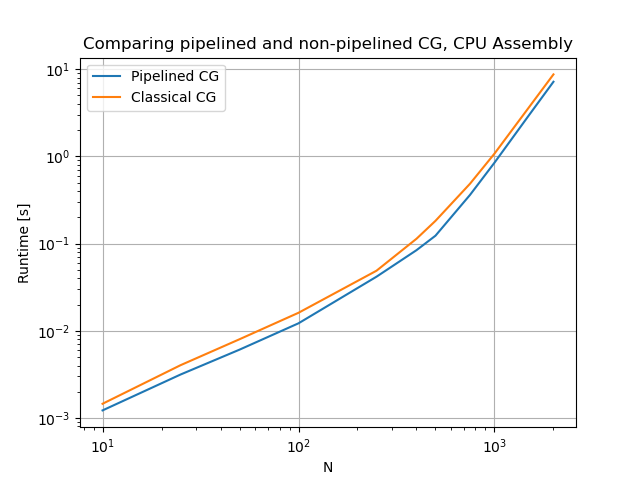
\includegraphics[scale=0.8]{plots/1comp_dual.png}

(The x-axis is wrongly labeled as \(N\) here, it should read \(\sqrt{N}\).) \\
Depending on the size of \(N\), we see performance increases between \(10-40\%\), which is quite respectable. The best gain in that respect is received for `middling' \(N\) that are neither too high nor too low.

\end{document}
